\chapter{Realizacja projektu}
%TODO Bardziej informatywny tytuł.

%TODO Ogólnie to zacząłbym od koncepcji systemu, omówieniu symulatorów, potem te narzędzia i potem realizacji.

W niniejszym rozdziale zostanie opisana implementacja systemu służącego do testowania algorytmów wizyjnych z użyciem symulatora Euro Truck Simulator 2. 
Do stworzenia systemu użyto następujących elementów:
\begin{itemize}
\item Python 3.7 -- język programowania wysokiego poziomu ogólnego przeznaczenia,
\item gra Euro Truck Simulator 2,
\item SDK (ang. \textit{Software Development Kit}) udostępnione przez twórców gry,
\end{itemize}
a także biblioteki: 
\begin{itemize}
\item OpenCV 3.1.3 -- biblioteka zawierająca funkcje do cyfrowego przetwarzania obrazów,
\item threading -- biblioteka wspierająca programowanie wielowątkowe,
\item libWnck -- biblioteka zapewniająca komunikację ze środowiskiem graficznym (Window Navigator Construction Kit),
\item uinput -- biblioteka pozwalająca symulować kontroler do sterowania grą.
\end{itemize}

System jest opracowany do działania na systemie Ubuntu 18.04 LTS wraz ze środowiskiem graficznym GNOME.
%TODO system, system.,

\section{Euro Truck Simulator 2}

Euro Truck Simulator 2 jest to symulator jazdy ciężarówką opracowany przez czeskie studio SCS Software.
Pozwala on na jazdę wybranym modelem ciężarówki przez wiele dróg Europy oraz na realizację zleceń na przewóz towarów. 
Z uwagi na charakter niniejszej pracy, interesującymi elementami gry jest wysoka jakość grafiki, wiernie odwzorowująca otaczający świat, w tym zestaw znaków i linii drogowych charakterystycznych dla poszczególnych krajów. 
Kolejnym elementem który opowiada za wyborem tego symulatora jest otwartość na wszelkie modyfikacje. 
Twórcy gry udostępnili API (ang. \textit{Application Programming Interface}), a także konsolę, za pomocą której można na bieżąco modyfikować parametry gry takie jak czas, prędkość gry lub pogodę.
Alternatywnym symulatorem, który również był brany pod uwagę jest American Truck Simulator 2, jednak jest on kalką symulatora opisywanego w tej sekcji ze zmienionym obszarem gry z równie dobrą grafiką i wsparciem dla programistów. %TODO sekcko
Kolejną możliwością są gry z serii Grand Theft Auto, jednak na ich niekorzyść wskazywało gorsze wsparcie dla programistów, a także niewspółmierne zużycie zasobów do uzyskiwanej jakości obrazu (GTA V) lub niskie zużycie zasobów przy niskiej jakości obrazu (GTA: San Andreas). 
Fakt, że jest to symulator ciężarówki, a nie samochodu osobowego w żaden sposób nie wpływa na podejście do problemu systemów wizyjnych, ponieważ po pierwsze, istnieją aplikacje wspomagające kierowcę samochodu ciężarowego, po drugie jeden z widoków w grze jest umieszczony w miejscu, które znajduje się na wysokości lusterka samochodowego.

Wspomniana konsola dostępna w grze pozwala na błyskawiczną zmianę warunków w symulatorze. 
Używając następujących komend można zmienić czas, pogodę oraz prędkość gry:

\begin{itemize}
\item g\_ set\_ weather x -- komenda zmieniająca pogodę. Gdy x jest równy 1, pogoda jest deszczowa, natomiast, gdy jest równy 0 pogoda jest słoneczna
\item g\_ set\_ time x -- komenda ustalająca godzinę w grze. W miejsce x należy podać godzinę w formacie hh,
\item warp x -- komenda zmieniająca prędkość gry. W miejsce x należy wpisać współczynnik. Liczba mniejsza od 1 zwolni grę, a większa przyspieszy.
\end{itemize}

%TODO Ten rozdział proszę przeredagować na omówienie poszczególnych symulatorów + końcowy wybór i uzasadnienie. Zasadniczo bedzie to przeredagowanie istniejęcej treści.
%TODO inna sprawa to wspomnieć o licenji ?

\section{Architektura systemu}

Z uwagi na dydaktyczną wartość opisywanego systemu ważnym elementem jest łatwość implementacji systemu analizy obrazu dla przyszłych użytkowników. %TODO powt. systemu
Z tego powodu zdecydowano się na implementację wieloprocesową, której schemat jest widoczny na rysunku \ref{fig:arch}, w której jeden z procesów jest odpowiedzialny za analizę obrazu i wypracowanie sterowania, a pozostałe za poprawne przechwycenie obrazu z gry i "wstrzyknięcie" wypracowanego sterowania do gry. %TODO to wstrzyknięcie średnio pasuje

\begin{figure}
  \centering
  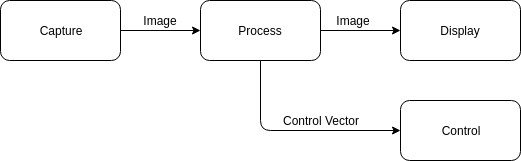
\includegraphics[width=13cm]{img/architektura.png}
  \caption{Schemat architektury aplikacji}
  \label{fig:arch}
\end{figure}

Poszczególne procesy są połączone kolejkami, za pomocą których transportowane są dane pomiędzy nimi. 
W przypadku opisywanej aplikacji w kolejkach umieszczane są obrazy wejściowe i wyjściowe z procesu $Process$, a także wektor sterowań do procesu $Control$. 
Szybkość działania aplikacji jest zależna od wielu czynników. 
Głównym elementem warunkującym jest czas przetwarzania obrazu w bloku $Process$. 
W~zależności od liczby obrazów czekających na przetworzenie w kolejce zmieniany jest interwał pomiędzy poszczególnymi przechwyceniami obrazu w bloku $Capture$. 
Uniezależnienie przechwytywania obrazu od zapełnienia kolejki spowodowałoby szybkie jej przepełnienie i zabicie aplikacji przez system.  %TODO "zabicie" potoczne
Końcowe procesy tj. $Display$ i $Control$ nie wymagają wyzwalania w zależności od czasu przetwarzania obrazu, ponieważ wykonują się bardzo szybko (poniżej 10ms).

Używana biblioteka \textit{multiprocessing}\cite{S2} pozwala na tworzenie podprocesów. 
Korzyść uzyskana z tego tytułu względem korzystania z wątków polega na tym, że program napisany z użyciem tej biblioteki jest w pełni w stanie korzystać z wielu procesorów lub rdzeni komputera. %TODO styl + mógłby Pan to nieco rozwinąć

%TODO W kolejnych dodać nazwy bloków
\subsection{Przechwytywanie obrazu}
\label{sec:mechanism}
Optymalnym rozwiązaniem byłoby przechwytywanie obrazu wprost z pamięci symulatora, lecz niestety póki co nie istnieją metody pozwalające na takie rozwiązanie. %TODO chyba raczej API tego nie udostępnia.
W procesie $Capture$ realizowane są dwa podzadania. 
Pierwsze polega na znalezieniu i aktywowaniu okna symulatora. 
Ma to na celu zapobiegnięcie przechwycenia obrazu, gdy okno gry jest przysłonięte przez inną aplikację lub zminimalizowane. 
Następnie, za pomocą biblioteki \texttt{libwnck} odczytanie współrzędnych okna gry (współrzędne górnego rogu, szerokość i wysokość). 
Dopiero, gdy jest zapewniony poprawny obraz do przechwycenia jest to robione, a obraz w postaci macierzy o wymiarach 1024x768x3 jest wkładany w kolejkę i wysyłany do procesu przetwarzania i analizy obrazu. %TODO styl. - to jest to robione + wkładany (potoczne)
Jednorazowe przechwycenie okna zajmuje średnio około 10ms.

\subsection{Przetwarzanie i analiza obrazu}

Jeśli kolejka wejściowa do procesu nie jest pusta, to obraz jest z niej pobierany, a następnie w zależności od wybranego algorytmu (detekcja linii, detekcja znaków) jest przetwarzany. 
Poszczególne opisy zaimplementowanych algorytmów znajdują się w sekcjach TODO: numery sekcji z opisem algorytmów. %TODO to się \ref używa
Istotne jest, aby po skończeniu obróbki obrazu i wypracowaniu sterowania włożyć obraz z zaznaczonym wynikiem przetwarzania i wektor sterowań do kolejki. %TODO pot. obróbki, włożyć do kolejki

\subsection{Symulacja kontrolera}

Euro Truck Simulator 2 pozwala użytkownikowi na sterowanie ciężarówką za pomocą licznych kontrolerów. 
Może to być klawiatura, klawiatura w zestawie z myszką komputerową, kierownica lub gamepad. 
W systemach UNIX-owych każde urządzenie wejściowe podpięte do komputera jest widoczne jako plik w lokalizacji $\backslash dev\backslash input\backslash $. 
Urządzenia generują zdarzenia (ang. \textit{event}), które są przesyłane do korzystających z nich aplikacji.
Biblioteka $uinput$ pozwala na zasymulowanie dowolnego kontrolera i sterowanie nim programowo. 
Na potrzeby opisywanej aplikacji stworzono kontroler, która posiada trzy osie analogowe: kierownica, pedał gazu i pedał hamulca. 
Dodatkowo, w~celu umożliwienia programowej kontroli nad konsolą, kontroler posiada pełen zestaw klawiszy z układu QWERTY. %TODO kontroler, kontroli
Podczas inicjalizacji aplikacji jest inicjalizowany kontroler, tak, aby przed rozpoczęciem właściwej rozgrywki i przetwarzania obrazu gra wykryła poprawnie urządzenie do sterowania. %TODO powt inicjalizacji
Klasa $Control$ posiada metodę $emit$, która odpowiada za wygenerowanie zdarzenia z odpowiednimi wartościami sterowania. 
Podczas wykonywania tej metody jest sprawdzane czy okno z grą jest aktywne, ponieważ w przypadku wyemitowania sterowania przy nieaktywnym oknie, sterowanie nie będzie poprawnie zintepretowane przez symulator. %TODO emitowanie sterowania to też średnie określenie

\subsection{Wyświetlanie rezultatów}

Wyświetlanie rezultatów jest opcjonalne. 
Jest realizowane w osobnym procesie ze względu na ustaloną architekturę systemu, która zakłada, że w procesie odpowiedzialnym za przetwarzanie obrazu będzie realizowane tylko przetwarzanie. %TODO przeredagować - procesie, procesie, przetwarzanie, przetwarzanie
Wyświetlanie obrazu jest realizowane za pomocą funkcji biblioteki OpenCV $imshow()$.


\section{Opis implementacji algorytmów wizyjnych użytych w symulatorze}

W tej sekcji zostaną opisane algorytmy służące do przetestowania działania frameworku stworzonego w ramach pracy magisterskiej. %TODO sekcji ! i może bez framework
Cele jakie są postawione przed zaimplementowanym frameworkiem to: przetwarzanie obrazu w czasie rzeczywistym lub do niego zbliżonym oraz dostęp do wirtualnego kontrolera symulowanego w ramach aplikacji. %TODO to drugie nie do końca jasne

\subsection{Algorytm detekcji linii}

W symulatorze Euro Truck Simulator 2 występuję typy dróg z każdego kraju Europy. 
Zaczynając od szerokich autostrad, poprzez drogi ekspresowe na wąskich i krętych drogach w Alpach kończąc. Zaimplementowany algorytm jest przeznaczony do detekcji linii na drogach, których krzywizna łuku nie jest duża. 
Przykładowy obraz wejściowy jest widoczny na rysunku \ref{fig:inputimg}. %TODO lepiej powtórzyć, bo takie odwołanie kilkanaście stron wstecz źle działa. Ten S można zmniejszyć i dać dwa obok siebie.
Pierwszym krokiem jest konwersja przestrzeni barw z RGB do HSV. 
Wybranie składowej S jako obrazu poddawanego analizie (rys. \ref{fig:alg1_S}) pozwala uniezależnić się od pory dnia i pogody.

\begin{figure}
  \centering
  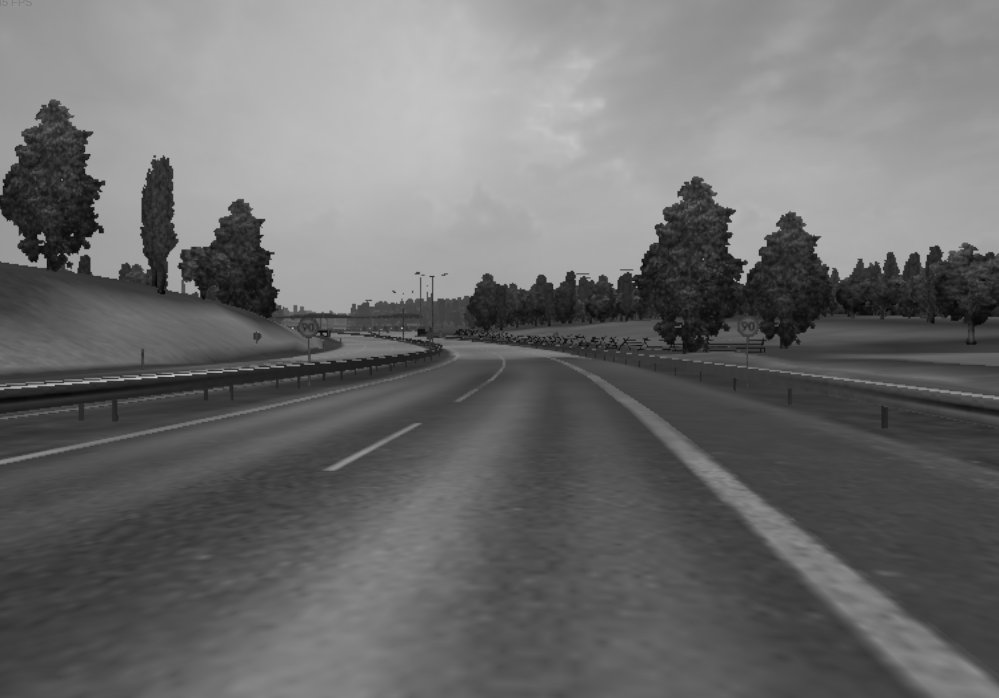
\includegraphics[width=13cm]{img/alg1_gray.jpg}
  \caption{Obraz wejściowy (składowa S)}
  \label{fig:alg1_S}
\end{figure}

Założenie, że obszar jezdni może znajdować się tylko na pewnym obszarze obrazu pozwala zaoszczędzić czas obliczeń. %TODO styl powt. obszar.
Po wybraniu ROI otrzymano obraz \ref{fig:alg1_roi}.
%TODO prosze skomentować na jakiej zasadzie to ROI

\begin{figure}[h]
	\centering
	\begin{subfigure}{0.35\textwidth}
		\centering
		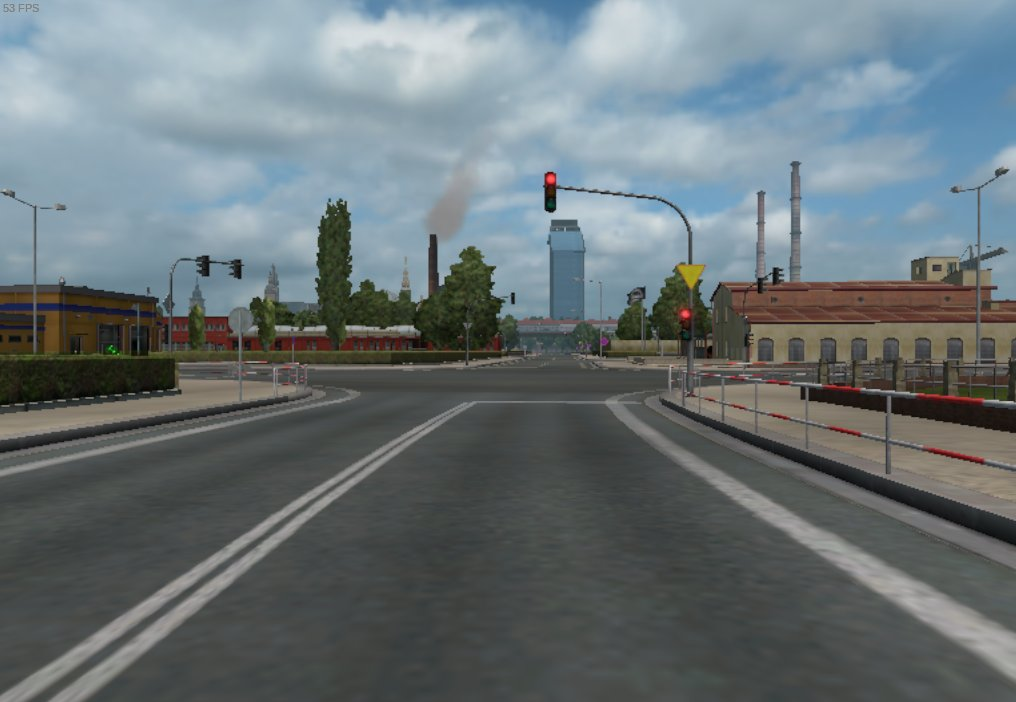
\includegraphics[width=6cm]{img/low_details.jpg}
		\subcaption{\label{fig:low_details}}
	\end{subfigure}
	\begin{subfigure}{0.35\textwidth}
		\centering
		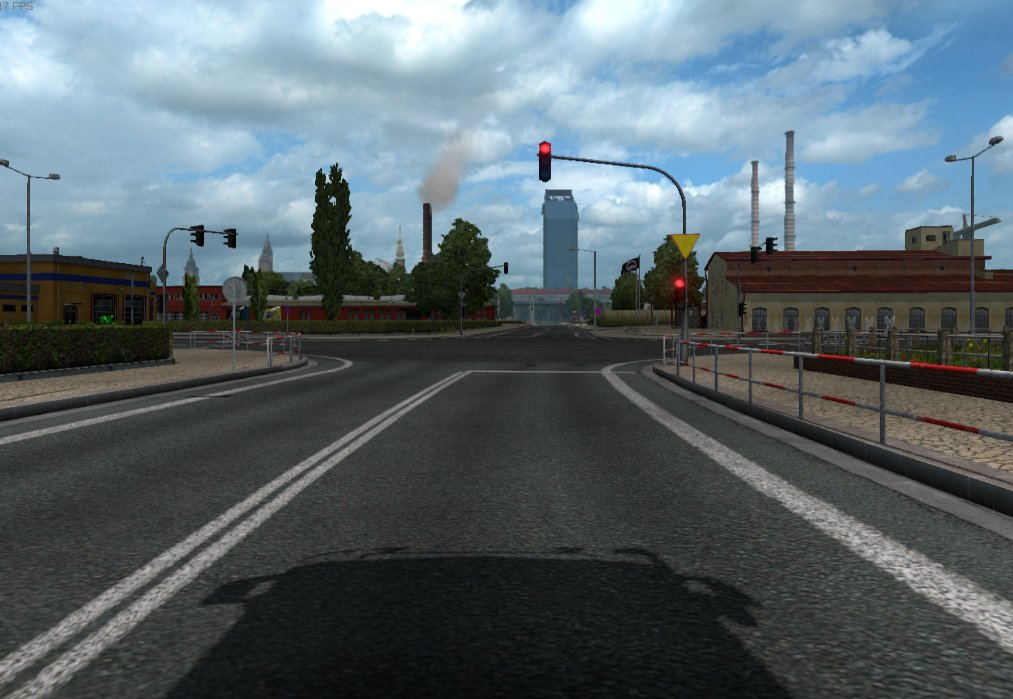
\includegraphics[width=6cm]{img/high_details.jpg}
		\subcaption{\label{fig:high_details}}
	\end{subfigure}
	
	\caption{\label{fig:details1}Porównanie niskich \protect\subref{fig:low_details} i wysokich \protect\subref{fig:high_details} ustawień grafiki symulatora}
\end{figure}

Kolejnym krokiem jest wykrycie krawędzi z użyciem filtru Canny'ego. 
Progi dobrane są eksperymentalnie. %TODO są -> zostały ? 
Należy zwrócić uwagę, że gra pozwala na ustalenie jakości grafiki. 
W związku z tym, każdorazowo po zmianie ustawień należy dobrać współczynniki filtru na nowo. 
Wraz ze wzrostem jakości grafiki poprawia się jej ostrość. %TODO trochę dziwnie to brzmi
Porównanie niskich i wysokich ustawień graficznych jest widoczne na rysunku \ref{fig:details1}. %TODO sformułowanie niskie i wysokie ustawienie grafiki jest potoczne
Kolejną rzeczą wartą uwagi przy wyborze ustawień grafiki jest to, że zarówno praca zaimplementowana w tej pracy jak i gra są uruchamiane na jednej maszynie. %TODO nieco inaczej ująć.
W związku z tym wybranie niskich ustawień grafiki pozwoli na przekazanie zasobów obliczeniowych do aplikacji.
%TODO może nie w tym miejscu, ale jakaś anaiza komentarz jak ta jakość wypływa na sposób działania algorytmów.

\begin{figure}
  \centering
  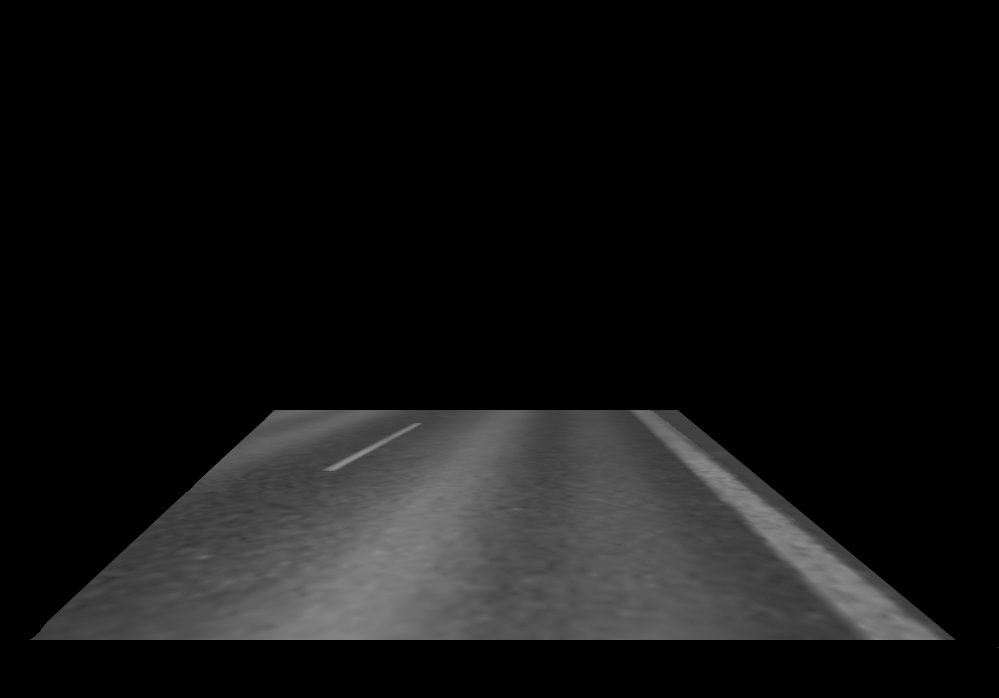
\includegraphics[width=13cm]{img/alg1_roi.jpg}
  \caption{Wyznaczone ROI, na którym można spodziewać się linii}
  \label{fig:alg1_roi}
\end{figure}

Na obrazie krawędzi, za pomocą transformaty Hougha wykonywana jest detekcji linii prostych. 
Linie fałszywe (linie nie będące liniami na jezdni) można odrzucić badając ich parametr $\theta$. %TODO orientację ?
Właściwe linie będą pochylone pod odpowiednim kątem. 
Dla opisywanego przypadku właściwym zakresem kąta nachylenia linii jest $\theta < 1.3rad$ dla linii po lewej i $\theta > 2rad$ dla krawędzi prawej. %TODO powt. właściwe

W celu zaoszczędzenia czasu obliczeń i poprawienia sprawności algorytmu założono, że rezultatem powinna być linia dla każdej z krawędzi jezdni. Jeśli wykryto kilka linii, których parametry są zbliżone, dalszej analizie poddawana jest tylko jedna z nich (rys. \ref{fig:alg1_res}).
%TODO no ale która ?

Aby wygenerować sterowanie bada się punkt przecięcia wykrytych linii (biały okrąg na rys. \ref{fig:alg1_res}). Zakładając, że kamera jest ustawiona w osi ciężarówki można przyjąć, że każde odchylenie punktu przecięcia wykrytych linii powinno implikować ruch kierownicą.
%TODO nie za bardzo jasne od czego to odchylenie...

\begin{figure}
  \centering
  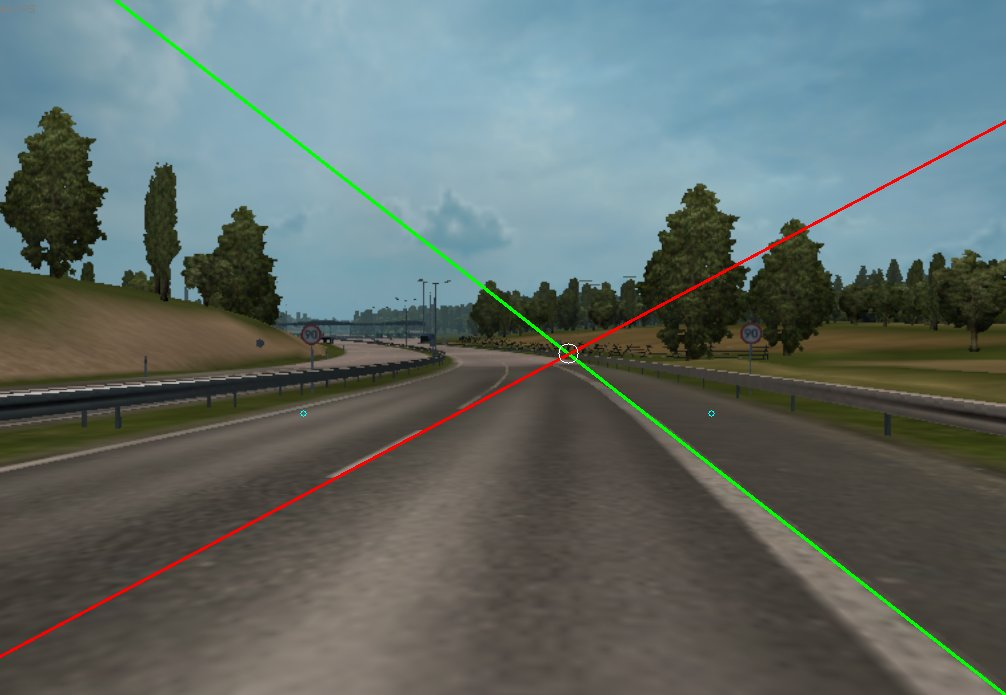
\includegraphics[width=13cm]{img/alg1_res.jpg}
  \caption{Rezultat działania algorytmu}
  \label{fig:alg1_res}
\end{figure}

Średni czas obliczeń potrzebny do przetworzenia jednej klatki wyniósł 59ms, co daje możliwość przetworzenia 17 klatek na sekundę. 
Jest to wydajność wystarczająca, aby zapewnić stabilność całości algorytmu, ponieważ ciężarówka była w stanie utrzymać się przy stałej prędkości na pasie ruchu długim na ok. 500m.
%TODO - a potem co ? Gleba ?

\subsection{Sytuacje potencjalnie problematyczne}
Jak wspomniano w sekcji \ref{sec:lane_detection} wymagane jest poprawne działanie algorytmu przy zmiennych warunkach oświetlenia i pogody. %TODO sekcja !
Symulator oferuje możliwość zmiany tych parametrów poprzez konsolę. 
Algorytm wykazał skuteczność zarówno przy zmianie godziny gry na późniejszą oraz dodaniu deszczu (rys. \ref{fig:alg1_late} i rys. \ref{fig:alg1_rain})

\begin{figure}
  \centering
  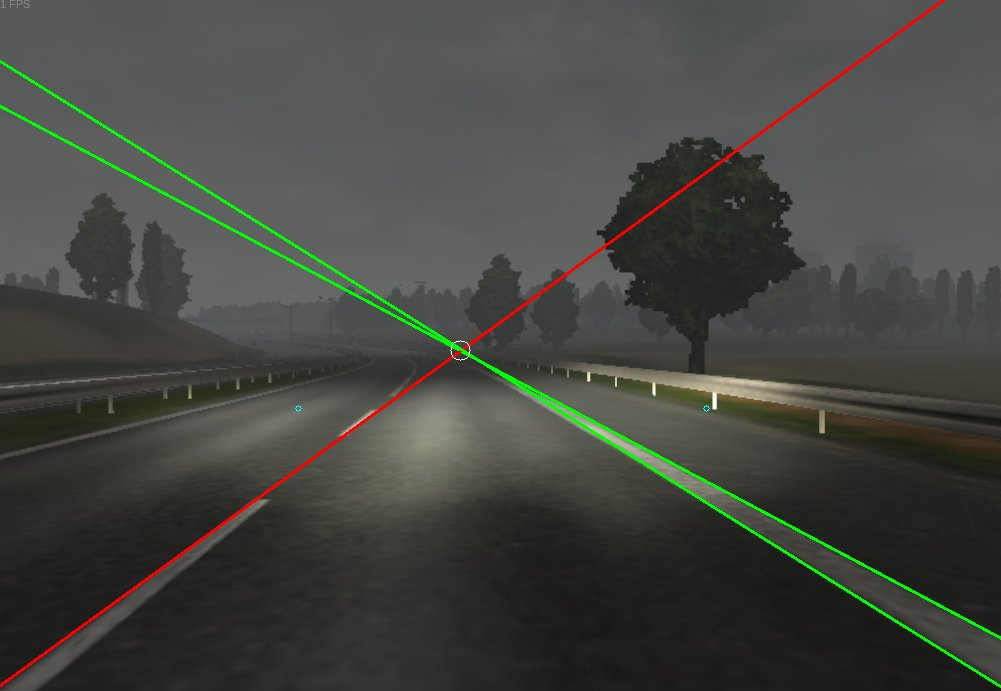
\includegraphics[width=13cm]{img/alg1_late.jpg}
  \caption{Działanie algorytmu podczas trudnych warunków oświetleniowych}
  \label{fig:alg1_late}
\end{figure}

\begin{figure}
  \centering
  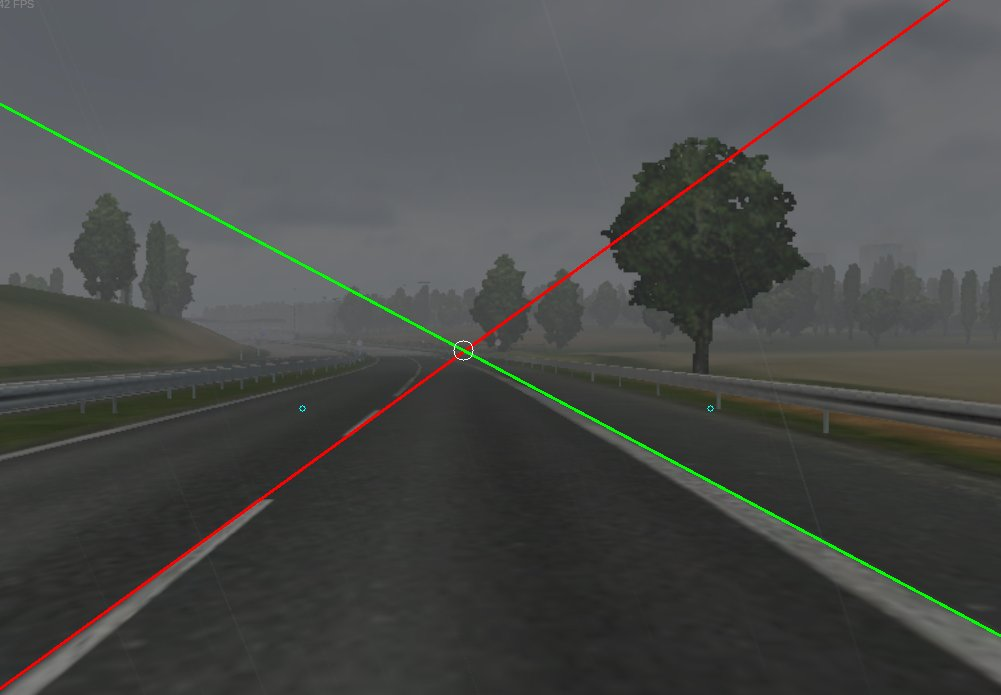
\includegraphics[width=13cm]{img/alg1_rain.jpg}
  \caption{Działanie algorytmu podczas deszczu}
  \label{fig:alg1_rain}
\end{figure}

%TODO te rysunki moglby być mniejsze.
%TODO No i ciekawi mnie co się dzieje po tych 500m, może jakieś demo. No i jaki może być łuk, bo niewielki powinien zadziałać..

\subsection{Algorytm detekcji czerwonych świateł drogowych} %TODO tu i niżej uwaga o światłach drogowych

Kolejnym algorytmem testowym, który został zaimplementowany w ramach pracy jest uproszczona wersja algorytmu opisanego w sekcji \ref{sec:tl}. %TODO sekcja
Przykładowy obraz wejściowy znajduje się na rysunku \ref{fig:alg2_input}. 
Dają się tam zauważyć dwa sygnalizatory świetlne, a także kilka znaków drogowych. 
Sceneria została dobrana tak, aby jednocześnie sprawdzić odporność algorytmu na znaki zawierające czerwoną barwę.

Pierwszym krokiem opisywanej metody jest wyznaczenie kandydatów na światła drogowe. 
Dobierając eksperymentalnie współczynniki progowania ustalono, że światło czerwone będzie spełniać poniższe warunki:
\begin{equation}
\label{eq:tl}
R>180 \wedge 0 \geq R<100 \wedge B < 120
\end{equation}

gdzie: $R, G, B$ oznaczają wartości składowych w przestrzeni RGB.

Aby zapewnić, że inne obiekty spełniające warunek \ref{eq:tl} wykonano operację erozji i dylatacji zwaną również otwarciem morfologicznym. %TODO czegoś tu brakuje.
Otrzymany obraz indeksuje się. %TODO poddawany jest indeksacji.
Iterując po każdym z wyznaczonych elementów można sprawdzić jego powierzchnię i proporcje, które muszą spełniać pewne warunki, żeby zostać uznane za światło drogowe.
%TODO bardziej konkretnie niż pewne.

Aby zmodyfikować algorytm tak, by wykrywał światło zielone lub pomarańczowe należy zmienić wartości progów w warunku \ref{eq:tl}. 
Do indeksacji kandydatów wykorzystano funkcję biblioteki OpenCV $connectedComponentsWithStats()$, która zwraca listę obiektów wraz z ich statystykami.

\begin{figure}
  \centering
  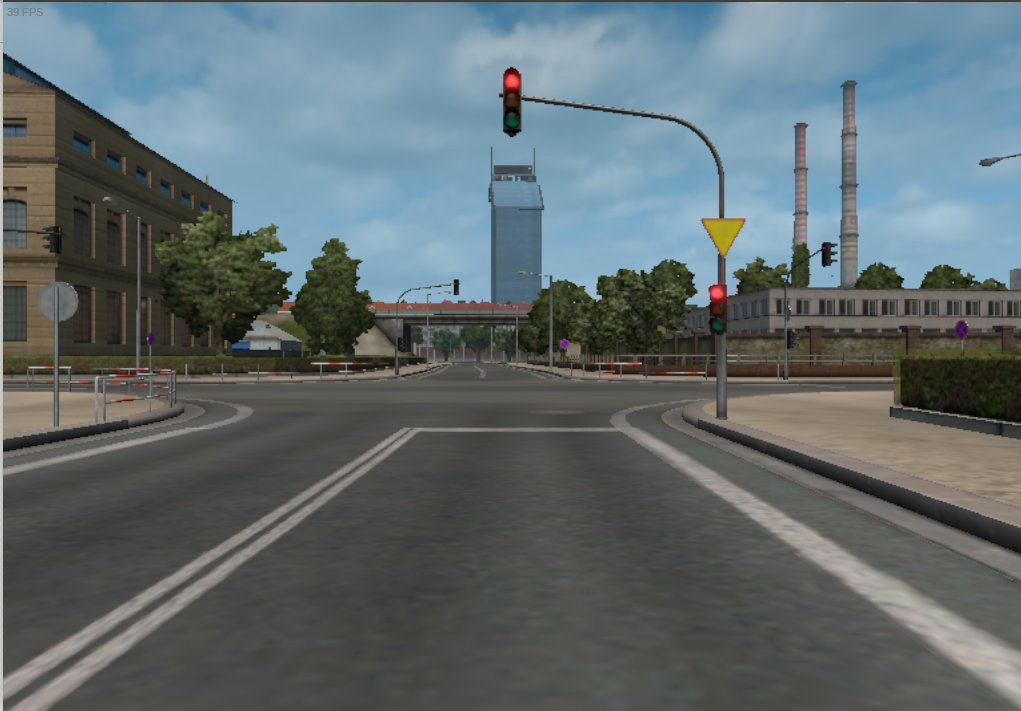
\includegraphics[width=13cm]{img/alg2_input.jpg}
  \caption{Przykładowy obraz wejściowy algorytmu}
  \label{fig:alg2_input}
\end{figure}

\begin{figure}
  \centering
  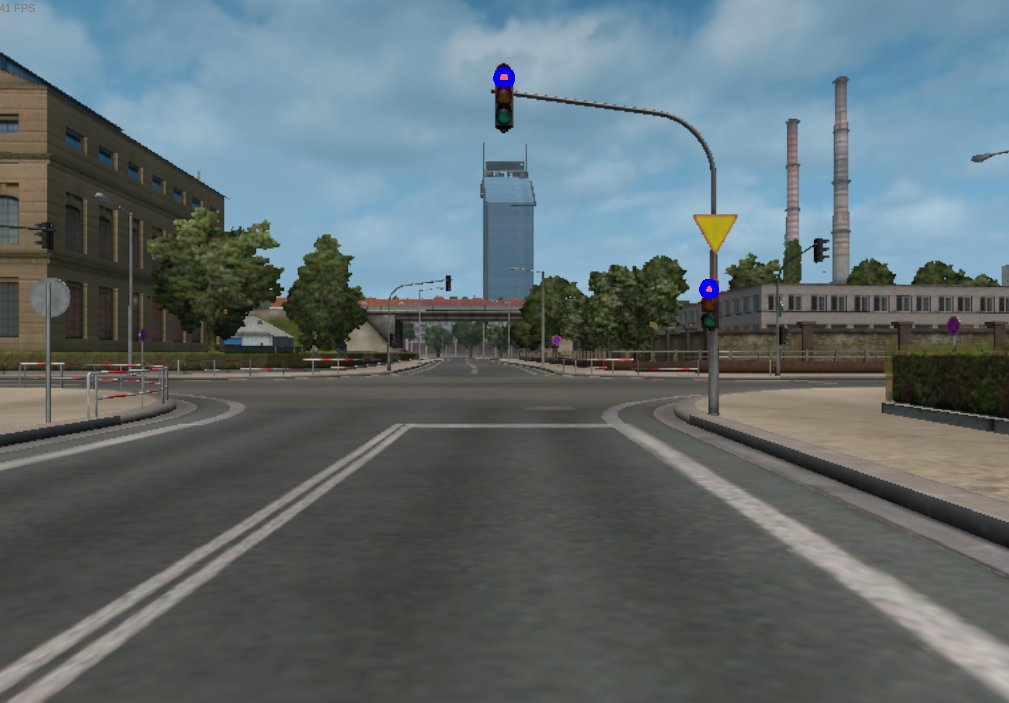
\includegraphics[width=13cm]{img/alg2_res.jpg}
  \caption{Wykryte dwa światła czerwone}
  \label{fig:alg2_res}
\end{figure}

\subsection{Sytuacje potencjalnie problematyczne}
Jak w przypadku każdego z omawianych algorytmów problemem jest zmiana warunków oświetleniowych oraz pogodowych. 
Nie można jak w przypadku algorytmu detekcji pasa ruchu uniezależnić się od zmian oświetlenia poprzez zastosowanie konwersji do przestrzeni HSV, ponieważ istotną rolę odgrywa tu barwa. %TODO no teoretycznie można - H... nie próbował Pan pewnie.
Z uwagi na to, że światła drogowe emitują światło, w czasie warunków słabej widoczności i deszczu algorytm poprawnie wykrywał czerwone światło (rys. \ref{fig:alg2_rain} i rys. \ref{fig:alg2_late}).

\begin{figure}
  \centering
  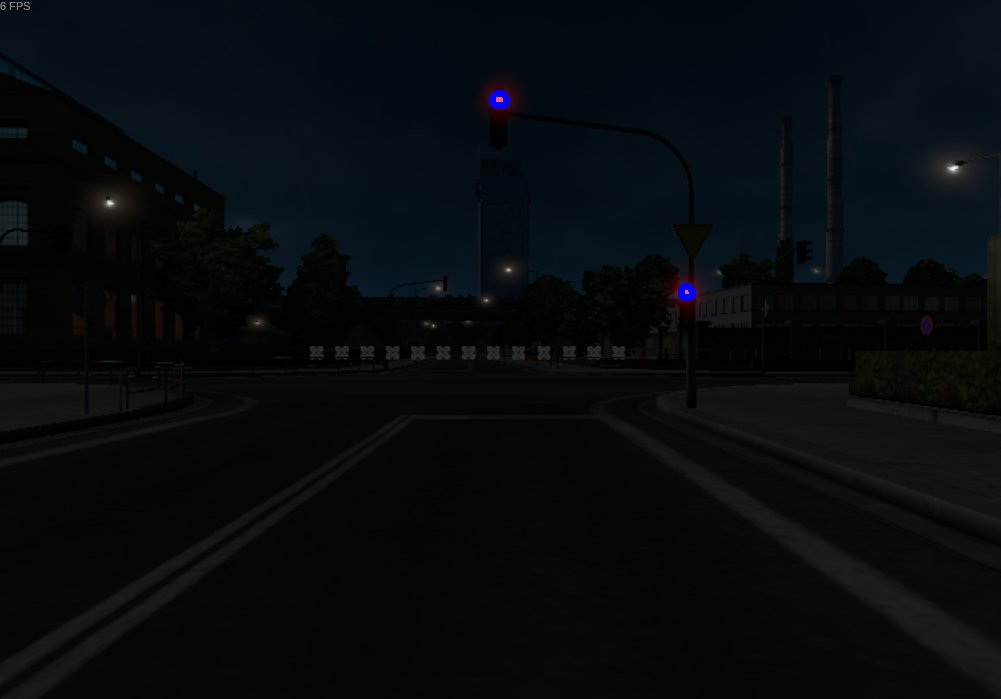
\includegraphics[width=13cm]{img/alg2_late.jpg}
  \caption{Wykryte światła drogowe w warunkach słabego oświetlenia}
  \label{fig:alg2_late}
\end{figure}

\begin{figure}
  \centering
  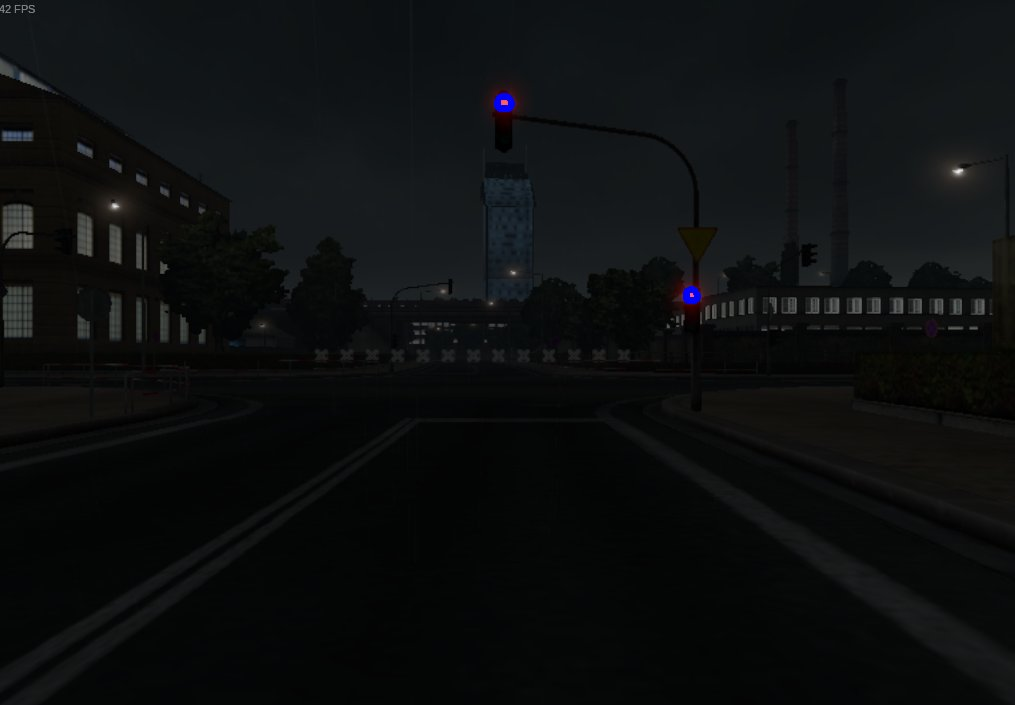
\includegraphics[width=13cm]{img/alg2_rain.jpg}
  \caption{Wykryta sygnalizacja świetlna podczas deszczu} %TODO o tu Pan użył sygnalizacja
  \label{fig:alg2_rain}
\end{figure}

%TODO a z tym było jakieś sterowanie związane ?

\subsection{Detekcja samochodu poprzedzającego}
Ostatnim algorytmem, który został zaimplementowany w ramach tej pracy była detekcja samochodów poprzedzających na drodze z użyciem detektora symetrii. 
Implementacja bazuje na algorytmie opisanym w sekcji \ref{sec:car_general}. %TODO sekcji

\begin{figure}
  \centering
  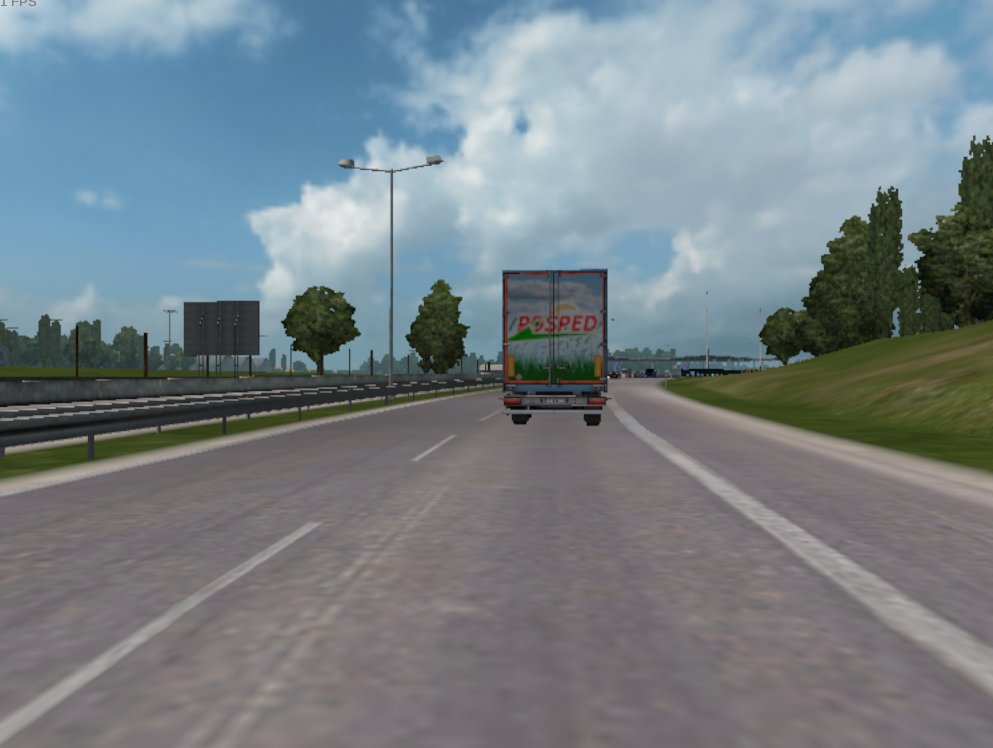
\includegraphics[width=13cm]{img/alg3_input.jpg}
  \caption{Przykładowy obraz wejściowy algorytmu detekcji samochodu poprzedzającego}
  \label{fig:alg3_input}
\end{figure}

Zaimplementowany algorytm operuje na obrazach w skali szarości. %TODO styl. operuje
Przykładowy obraz wejściowy jest pokazany na rysunku \ref{fig:alg3_input}. 
Daje się na nim zauważyć ciężarówkę poprzedzającą samochód. 
Celem działania algorytmu jest poprawne wykrycie symetrii na tyle naczepy samochodu.

\begin{figure}
  \centering
  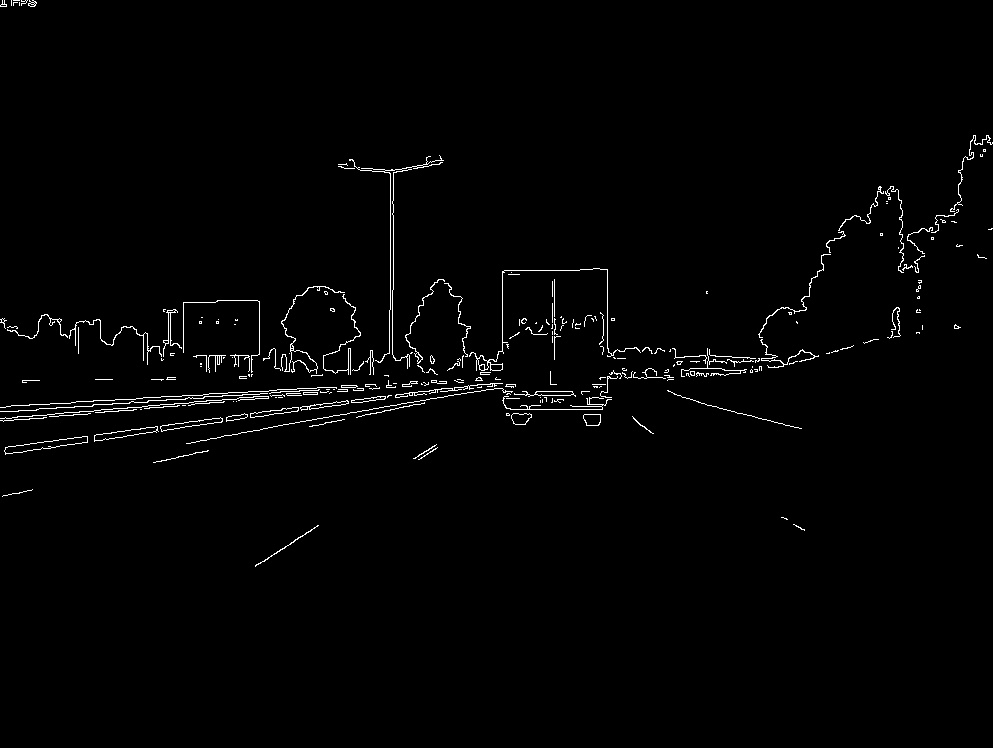
\includegraphics[width=13cm]{img/alg3_canny.jpg}
  \caption{Obraz wejściowy po detekcji krawędzi. Widoczna symetria w układzie krawędzi poprzedzającej naczepy}
  \label{fig:alg3_canny}
\end{figure}

Pierwszym krokiem jest filtracja z użyciem filtru Canny'ego. 
Progi filtru są dobierane eksperymentalnie każdorazowo po zmianie ustawień graficznych symulatora. %TODO jak wcześniej - o tych ustawieniech nieco więcej.
Efekt filtracji jest widoczny na rysunku \ref{fig:alg3_canny}.

Następnie wyznaczając linie skanu sprawdzana jest symetria obrazów w sposób opisany w sekcji \ref{sec:car_general}. %TODO sekcji
Na każdej z linii skanu wyznaczane są maksima, które wskazują na istnienie osi symetrii. 
Rezultaty detekcji są przedstawione na rysunkach \ref{fig:alg3_res1} i \ref{fig:alg3_res2}. 
Daje się zauważyć znaczna liczba detekcji fałszywych. 
Prawdopodobnie wynika to między innymi z faktu, że w symulatorze obiekty infrastruktury mają bardziej równomierny i symetryczny kształt.
%TODO ogólnie mam wrażenie, że akurat ta metoda jest kiepska.


\begin{figure}
  \centering
  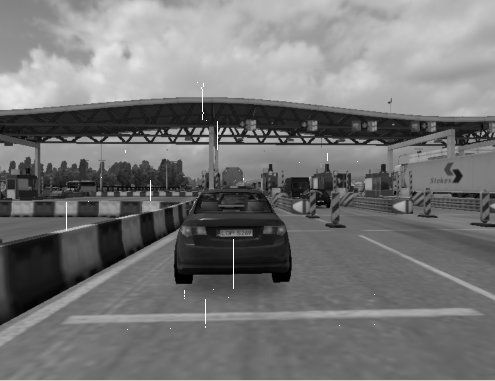
\includegraphics[width=13cm]{img/alg3_res.jpg}
  \caption{Rezultat detekcji samochodu osobowego. Widoczne liczne fałszywe detekcje.}
  \label{fig:alg3_res1}
\end{figure}

\begin{figure}
  \centering
  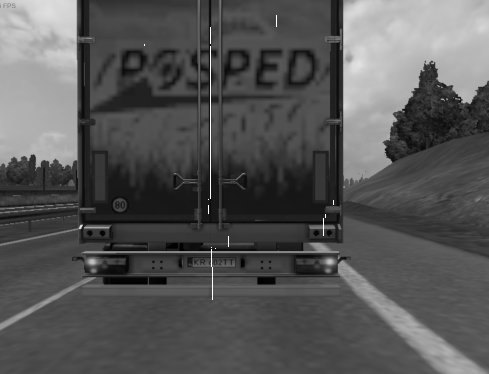
\includegraphics[width=13cm]{img/alg3_res2.jpg}
  \caption{Poprawna detekcja naczepy samochodu ciężarowego}
  \label{fig:alg3_res2}
\end{figure}

Sprawdzono również zachowanie algorytmu w trudnych warunkach pogodowych i słabego oświetlenia. 
Samochód korzysta ze świateł mijania, więc najbliższe otoczenie jest dobrze widoczne (rys. \ref{fig:alg3_rain_late}. 
W tym przypadku również pojawiają się fałszywe detekcje.

\begin{figure}
  \centering
  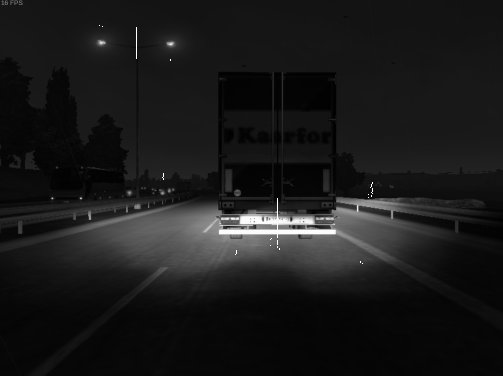
\includegraphics[width=13cm]{img/alg3_res3.jpg}
  \caption{Poprawna detekcja naczepy samochodu ciężarowego w trudnych warunkach oświetleniowych i pogodowych}
  \label{fig:alg3_rain_late}
\end{figure}

Obliczanie wskaźnika symetrii jest operacją bardzo czasochłonną. 
Średni czas przetworzenia jednej klatki to 5.45 sekundy. 
Oprócz dużej ilości obliczeń może to być spowodowane mało wydajną implementacją w Pythonie. 
Implementacja w języku C++ prawdopodobnie przyniosłaby lepsze efekty.
%TODO a można to zintegrować z C++ ?

%TODO czy tu było jakieś sterowanie ?

\section{Badania wydajności aplikacji}

Istotną rzeczą jest wydajność całej aplikacji. 
Powinna ona działać bez widocznych opóźnień, to znaczy, że po przechwyceniu obrazu z symulatora w możliwie najkrótszym czasie powinno zostać wygenerowane sterowanie. 
Jest to zapewnione poprzez mechanizm opisany w sekcji \ref{sec:mechanism}. %TODO sekcja
Eksperymentalnie dowiedziono, że liczba elementów w kolejkach, zwłaszcza w kolejce pomiędzy modułem $Capture$, a $Process$ nie powinna przekraczać 50. %TODO dowiedziono -> sprawdzono
Powyżej tej wartości daje się zauważyć widoczne opóźnienie reakcji systemu sterującego samochodem. 
Na wykresie przedstawiono rozmiar kolejki w kolejnych iteracjach programu podczas działania systemu wizyjnego odpowiedzialnego za detekcję czerwonego światła.

\begin{figure}
  \centering
  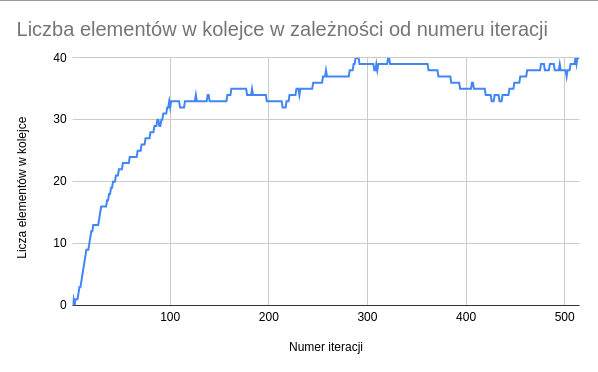
\includegraphics[width=13cm]{img/queue_stats.png}
  \caption{Rozmiar kolejki w trakcie działania programu}
  \label{fig:queue_stats}
\end{figure}

W trakcie implementacji kolejnych systemów wizyjnych używanych w pojazdach autonomicznych należy zwrócić uwagę na optymalizację kodu. 
Nie powinno się tworzyć wielu kopii obrazu w pamięci, a także, z uwagi na asynchroniczny charakter aplikacji,  używać komend typu $wait()$. 
Ważnym aspektem, który znacząco poprawił wydajność całości systemu było zastosowanie wektoryzacji, czyli wbudowanej w język programowania metody operowania na macierzach. 
W przypadku, gdy algorytm ze względu na swoją złożoność wykonywałby się zbyt długo, należy użyć komendy w konsoli symulatora udostępnionej przez twórców, która zmieni prędkość gry -- $warp x$, gdzie $x$ oznacza prędkość (1 - standardowa prędkość rozgrywki).

\section{Ewaluacja systemu}

Celem pracy było stworzenie aplikacji, która będzie w ramach przedmiotu Systemy i Algorytmy Percepcji Pojazdów Autonomicznych prowadzonego na II stopniu studiów stacjonarnych na kierunku Automatyka i Robotyka pozwalała w przyjazny użytkownikowi sposób na implementację i testowanie algorytmów wizyjnych stosowanych w pojazdach autonomicznych. 
Przykładowe algorytmy zaimplementowane w ramach tej pracy dowodzą, że jest to możliwe. 
Korzystanie z aplikacji w ramach zajęć jest zamienną formą w stosunku do korzystania ze zbiorów zdjęć np. KITTI. %TODO ref
Nie jest możliwym utworzenie $groundtruth$, aczkolwiek inną formą sprawdzenia czy dany algorytm działa poprawnie jest weryfikacja poprzez zachowanie ciężarówki w symulowanym świecie. %TODO może wygenerowanie wyników referencyjnych (ang. ground).
Opcjonalne jest generowanie sterowania na podstawie wyników z algorytmów wizyjnych. 
Końcowy użytkownik może tradycyjnie za pomocą klawiatury lub myszki sterować pojazdem i na bieżąco badać rezultaty osiągane przez algorytm.

Kolejnym etapem rozwoju projektu byłoby stworzenie prostego instalatora, który pobierze i zainstaluje wszystkie potrzebne biblioteki, a także skompiluje zmodyfikowane SDK udostępnione przez twórców. 
Możliwa jest także dalsza edycja SDK, poprzez umożliwienie odczytu pozostałych zmiennych gry oprócz aktualnej prędkości i stanu pauzy. 
Pełna lista parametrów jest dostępna w \cite{S3}. 
Elementem mocno rozbudowującym aplikację byłoby także generowanie danych radarowych na podstawie otoczenia samochodu w symulatorze. 
Póki co twórcy gry nie udostępniają takiej możliwości przez SDK.
%TODO radar, lidar...


\chapter{Podsumowanie}
Zgodnie z założeniami zrealizowano cele pracy. 
Dokonano ewaluacji przykładowych algorytmów wizyjnych, które mogłyby znaleźć zastosowanie w pojazdach autonomicznych, a także przetestowano ich działanie z użyciem zaimplementowanego frameworka. %TODO nie podoba mi się ten "framework".
Zdaniem autora przygotowany framework nadaje się do użycia w ramach zajęć dydaktycznych.
Pozwala w łatwy sposób modyfikować parametry obrazu takie jak natężenie światła, pogodę oraz liczbę otaczających pojazdów. 
%TODO no właśnie - nigdzie Pan nie opisał jak to działa - czy wybiera się gdzie się jedzie i inne parametry "świata".
%TODO czy można wielokrotnie odtwarzać tą samą "scenę" np. przejazd danym fragmentem...
Znaczącą przewagą systemu nad analizą pojedynczych zdjęć jest możliwość przetestowania algorytmów w sytuacjach dynamicznych. 
Zaimplementowana możliwość sterowania samochodem w symulatorze z pewnością pozwoli na rozbudowanie powstających algorytmów i sprawdzanie ich pod kątem wielu nowych aspektów takich jak np. optymalizacja kodu, by przyspieszyć jego wykonanie.
%TODO ja bym raczej stawiał na funkcjonalnści

%TODO Tu jeszcze wspomienie o części teoretycznej i póżniej o dodatku

